CP2K placeholder text.

What follows is a series of queries for particular kinds of questions of interest that were driven by the needs of CP2K as well as within the \acs{OLCF}.
This is not intended to be a form of definitive analysis to provide specific solutions to problems, but rather a means to create a few classes of representative queries that we expect to be of general use for any user code or system administration.
We start with some queries that require only the output from the compiler and thus are immediately compatible with the normal XALT workflow, then proceed to demonstrate the full power of the tool with a more complex query that makes use of all the different sources of information available to the tool.
However, all of these queries can be easily modified to work on different fields/attributes, combined, or broken apart in any number of ways, as well as made with or without the use of the code sampling frequencies obtained from user profiling to narrow the search space.

\subsection{Determining Use of System and User Libraries}
One of the bigger concerns for system administrators and vendors alike is determining which system resources, particularly that of libraries, are actively being used in applications so as to better direct their focus and efforts.
As such, it is valuable to query not just which libraries are linked in (which has already been done by previous tools like XALT), but also which functions within those libraries are actually getting called within user code.
To this end, we queried CP2K to discover which \ac{FFTW} functions were actually referenced in the code.
The results can be seen in Table~\ref{tab:fftw-funcs}

\begin{table}[htbp]
\caption{FFTW Subroutines Referenced}
\begin{center}
\begin{tabular}{|c|}
\hline
\textbf{Subroutine} \\
\hline
fftw31dm \\
\hline
fftw33d \\
\hline
fftw3\_compute\_rows\_per\_th \\
\hline
fftw3\_create\_3d\_plans \\
\hline
fftw3\_create\_guru\_plan \\
\hline
fftw3\_create\_plan\_1dm \\
\hline
fftw3\_create\_plan\_3d \\
\hline
fftw3\_destroy\_plan \\
\hline
fftw3\_do\_cleanup \\
\hline
fftw3\_do\_init \\
\hline
fftw3\_get\_lengths \\
\hline
fftw3\_workshare\_execute\_dft \\
\hline
fftw\_export\_wisdom\_to\_file \\
\hline
fftw\_import\_wisdom\_from\_file \\
\hline
sortint \\
\hline
\end{tabular}
\label{tab:fftw-funcs}
\end{center}
\end{table}

\begin{table}[htbp]
\caption{ScaLAPACK Subroutine Reference Locations}
\begin{center}
\begin{tabular}{|c|c|c|}
\hline
\textbf{File} & \textbf{Lines} & \textbf{Subroutine} \\
\hline
src/cp\_dbcsr\_cholesky.F & {103} & pspotrf \\
\hline
src/cp\_dbcsr\_cholesky.F & {105} & pdpotrf \\
\hline
src/cp\_dbcsr\_cholesky.F & {187} & pspotri \\
\hline
src/cp\_dbcsr\_cholesky.F & {189} & pdpotri \\
\hline
src/fm/cp\_cfm\_basic\_linalg.F & {411} & pzgetrf \\
\hline
src/fm/cp\_cfm\_basic\_linalg.F & {703} & pzgetrf \\
\hline
src/fm/cp\_cfm\_basic\_linalg.F & {736,737} & pzgetrs \\
\hline
src/fm/cp\_cfm\_basic\_linalg.F & {799,800} & pzgetrf \\
\hline
src/fm/cp\_cfm\_basic\_linalg.F & {812,813} & pzgetri \\
\hline
src/fm/cp\_cfm\_basic\_linalg.F & {818,819} & pzgetri \\
\hline
src/fm/cp\_cfm\_basic\_linalg.F & {882} & pzpotrf \\
\hline
src/fm/cp\_cfm\_basic\_linalg.F & {938} & pzpotri \\
\hline
src/fm/cp\_cfm\_basic\_linalg.F & {1147} & pztrtri \\
\hline
src/fm/cp\_cfm\_diag.F & {90,91} & pzheevd \\
\hline
src/fm/cp\_cfm\_diag.F & {121,122} & pzheevd \\
\hline
%src/fm/cp\_fm\_basic\_linalg.F & {300} & pdgetrf \\
%\hline
%src/fm/cp\_fm\_basic\_linalg.F & {1348} & pdgetrf \\
%\hline
%src/fm/cp\_fm\_basic\_linalg.F & {1383} & pdgetrs \\
%\hline
%src/fm/cp\_fm\_basic\_linalg.F & {1400,1401} & pdgesvd \\
%\hline
%src/fm/cp\_fm\_basic\_linalg.F & {1406,1407} & pdgesvd \\
%\hline
%src/fm/cp\_fm\_basic\_linalg.F & {1511} & pdtrtri \\
%\hline
%src/fm/cp\_fm\_basic\_linalg.F & {1576} & pdgeqrf \\
%\hline
%src/fm/cp\_fm\_basic\_linalg.F & {1580} & pdgeqrf \\
%\hline
%src/fm/cp\_fm\_basic\_linalg.F & {1640} & pdgetrf \\
%\hline
%src/fm/cp\_fm\_basic\_linalg.F & {1641,1642} & pdgetrs \\
%\hline
%src/fm/cp\_fm\_basic\_linalg.F & {1776,1777} & psgetrf \\
%\hline
%src/fm/cp\_fm\_basic\_linalg.F & {1779,1780} & pdgetrf \\
%\hline
%src/fm/cp\_fm\_basic\_linalg.F & {1804,1805} & psgetri \\
%\hline
%src/fm/cp\_fm\_basic\_linalg.F & {1810,1811} & pdgetri \\
%\hline
%src/fm/cp\_fm\_basic\_linalg.F & {1820,1821} & psgetri \\
%\hline
%src/fm/cp\_fm\_basic\_linalg.F & {1823,1824} & pdgetri \\
%\hline
%src/fm/cp\_fm\_cholesky.F & {75} & pspotrf \\
%\hline
%src/fm/cp\_fm\_cholesky.F & {77} & pdpotrf \\
%\hline
%src/fm/cp\_fm\_cholesky.F & {143} & pspotri \\
%\hline
%src/fm/cp\_fm\_cholesky.F & {145} & pdpotri \\
%\hline
%src/fm/cp\_fm\_cholesky.F & {211} & pdsygst \\
%\hline
%src/fm/cp\_fm\_diag.F & {359,360} & pdsyevd \\
%\hline
%src/fm/cp\_fm\_diag.F & {380,381} & pdsyevd \\
%\hline
%src/fm/cp\_fm\_diag.F & {552,553} & pdsyevx \\
%\hline
\end{tabular}
\label{tab:scalapack-funcs}
\end{center}
\end{table}

\subsection{Determining Use of Language/Compiler Features}
\begin{figure}
\begin{center}
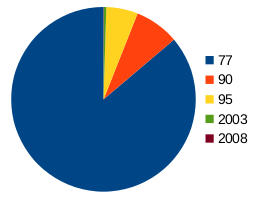
\includegraphics[width=0.4\textwidth]{images/cp2k-fortran-versions.png}
\end{center}
\caption{temp}
\label{fig:fortran-versions}
\end{figure}

\subsection{Finding OpenMP Regions Using Key Constructs}
%\subsection{Finding Unnecessary or Inefficient OpenMP Regions}

\subsection{Measuring Variable Use Within OpenMP Parallel Regions}

Figure~\ref{fig:openmp-refcount}

\begin{figure}
\begin{center}
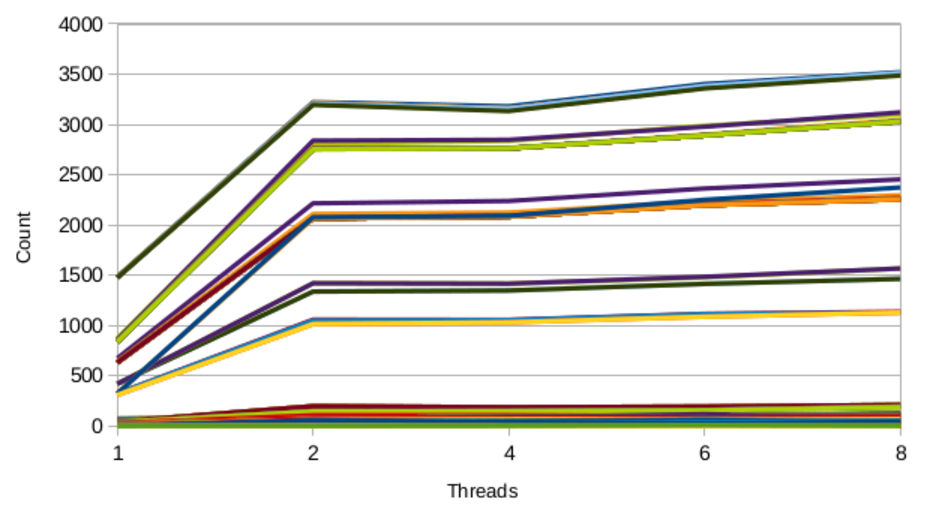
\includegraphics[width=0.4\textwidth]{images/cp2k-omp-inc-full.pdf}
\end{center}
\caption{Sampled reference counts to variables within OpenMP parallel regions}
\label{fig:openmp-refcount}
\end{figure}
